\subsection{Density}

\begin{definition}{Continuous Random Variable}{continuous-random-variable}
  $X$ is a continuous random variable if $\exists$ nonnegative $f$ (density of $X$)
  such that $\forall$ nice sets $B$,
  \[
    P(X\in B)=\int_B f(x)\dd{x}.
  \]
\end{definition}

\[
  1=P(-\infty<X<\infty)=\int_{-\infty}^{\infty}f(x)\dd{x}.
\]
\[
  F(x)=P(X\le x)=\int_{-\infty}^x f(y)\dd{y}.
\]

\subsection{Continuous Distributions}

\begin{definition}{Exponential Distribution}{exponential-distribution}
  Exponential distribution with parameter $\lambda>0$:
  \[
    f(x)=
    \begin{cases}
      \lambda e^{-\lambda x}, & x\ge0,            \\
      0,                      & \text{otherwise}.
    \end{cases}
  \]
\end{definition}

\begin{center}
  \begin{tikzpicture}[x=1.1cm,y=1.7cm]
    \draw[->] (-.7,0)--(4.3,0) node[right] {$x$};
    \draw[->] (0,-.15)--(0,1.3) node[above] {$f(x)$};
    \draw[blue,thick] (-.65,0)--(0,0);
    \draw[blue,thick,domain=0:4,samples=70] plot (\x,{exp(-\x)});
    \fill[blue] (0,1) circle[radius=1.5pt];
    \draw[blue,fill=white] (0,0) circle[radius=1.5pt];
    \node[left] at (0,1) {$\lambda$};
  \end{tikzpicture}
\end{center}

\begin{gather*}
  \int_{-\infty}^0 f(x)\dd{x}=0,\\
  \int_0^{\infty}f(x)\dd{x}
  =\lambda\int_0^{\infty}e^{-\lambda x}\dd{x}
  =\int_0^{\infty}e^{-u}\dd{u}=1.
\end{gather*}
For $t\ge0$,
\[
  P(X>t)=\int_t^{\infty}\lambda e^{-\lambda s}\dd{s}
  =\int_{\lambda t}^{\infty}e^{-u}\dd{u}=e^{-\lambda t}.
\]
For a continuous random variable,
\[
  0\le P(X=a)\le\int_{a-\varepsilon}^{a+\varepsilon}f(t)\dd{t}
  \longrightarrow0\qquad(\varepsilon\to0).
\]

\begin{definition}{Uniform Distribution}{continuous-uniform-distribution}
  $X$ uniformly distributed on the interval $(a,b)$, $a<b$:
  \[
    f(x)=
    \begin{cases}
      \dfrac1{b-a}, & a<x<b,            \\
      0,            & \text{otherwise}.
    \end{cases}
  \]
\end{definition}

\begin{center}
  \begin{tikzpicture}[x=1.2cm,y=1.6cm]
    \draw[->] (-1.6,0)--(3.2,0) node[right] {$x$};
    \draw[->] (0,-.2)--(0,1.4) node[above] {$f$};
    \draw[dashed] (-1,0)--(-1,1) (2.5,0)--(2.5,1);
    \draw[blue,thick] (-1,1)--(2.5,1);
    \draw[blue,thick] (-1.5,0)--(-1,0) (2.5,0)--(3,0);
    \foreach \x in {-1,2.5} {
      \draw[blue,fill=white] (\x,1) circle[radius=1.5pt];
      \fill[blue] (\x,0) circle[radius=1.5pt];
    }
    \node[below] at (-1,0) {$a$};
    \node[below] at (2.5,0) {$b$};
    \node[right] at (2.5,1) {$\dfrac1{b-a}$};
  \end{tikzpicture}
\end{center}

For $a<c<d<b$,
\[
  P(c<X<d)=\int_c^d f(x)\dd{x}=\frac{d-c}{b-a}.
\]

\begin{definition}{Normal Distribution}{normal-distribution}
  $X$ normal random variable with parameters: mean $\mu$, variance $\sigma^2>0$.
  Written $\mathcal{N}(\mu,\sigma^2)$,
  \[
    f(x)=\frac1{\sqrt{2\pi\sigma^2}}e^{-(x-\mu)^2/(2\sigma^2)}.
  \]
\end{definition}

\begin{center}
  \begin{tikzpicture}[x=.85cm,y=2cm]
    \draw[->] (-3.5,0)--(3.6,0) node[right] {$x$};
    \draw[dashed] (0,0)--(0,1);
    \draw[blue,thick,domain=-3.3:3.3,samples=100] plot (\x,{exp(-\x*\x/2)});
    \node[below] at (0,0) {$\mu$};
  \end{tikzpicture}
\end{center}

Symmetrical:
\[
  P(X>\mu)=P(X<\mu)=\frac12.
\]

\[
  P(X<a)=P(X\le a)
\]
by $\{X\le a\}=\underbrace{\{X<a\}\cup\{X=a\}}_{\text{disjoint}}$.

\subsection{Expectation}

\begin{definition}{Expectation of a Continuous Random Variable}{continuous-expectation}
  For $X$ with density $f$ and $\int_{-\infty}^{\infty}|x|f(x)\dd{x}<\infty$,
  \[
    E[X]=\int_{-\infty}^{\infty}xf(x)\dd{x}.
  \]
\end{definition}

\begin{example}[Uniform Expectation]
  For $X\sim\operatorname{Uni}(a,b)$,
  \[
    E[X]=\int_a^b xf(x)\dd{x}
    =\frac1{b-a}\int_a^b x\dd{x}=\frac{b+a}2.
  \]
\end{example}

\begin{example}[Exponential Expectation]
  For $X\sim\operatorname{Exp}(\lambda)$,
  \[
    E[X]=\int_0^{\infty}x\lambda e^{-\lambda x}\dd{x}.
  \]
  $u=\lambda x$, $\mathrm{d}u=\lambda\,\mathrm{d}x$:
  \begin{align*}
    E[X] & =\frac1\lambda\int_0^{\infty}ue^{-u}\dd{u}           \\
         & =\frac1\lambda\left(\left[-ue^{-u}\right]_0^{\infty}
    +\int_0^{\infty}e^{-u}\dd{u}\right)=\frac1\lambda.
  \end{align*}
\end{example}

\begin{example}[Normal Expectation]
  For $\mathcal{N}(\mu,\sigma^2)$:
  \[
    E[X]=\int_{-\infty}^{\infty}\frac1{\sqrt{2\pi\sigma^2}}
    xe^{-(x-\mu)^2/(2\sigma^2)}\dd{x}.
  \]
  For $\mathcal{N}(0,1)$:
  \[
    E[X]=\int_{-\infty}^{\infty}\frac1{\sqrt{2\pi}}xe^{-x^2/2}\dd{x}.
  \]
  \begin{center}
    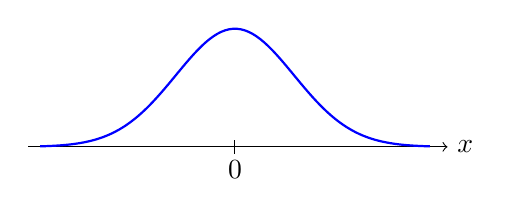
\begin{tikzpicture}[x=.75cm,y=1.5cm]
      \draw[->] (-3.5,0)--(3.6,0) node[right] {$x$};
      \draw (0,-.06)--(0,.06) node[below=4pt] {$0$};
      \draw[blue,thick,domain=-3.3:3.3,samples=100] plot (\x,{exp(-\x*\x/2)});
    \end{tikzpicture}
  \end{center}
  By symmetry, $E[X]=0$.

  For general $\mu,\sigma^2$? $y=x-\mu$:
  \begin{align*}
    E[X] & =\frac1{\sqrt{2\pi\sigma^2}}
    \int_{-\infty}^{\infty}ye^{-y^2/(2\sigma^2)}\dd{y}      \\
         & \quad+\frac\mu{\sqrt{2\pi\sigma^2}}
    \int_{-\infty}^{\infty}e^{-(x-\mu)^2/(2\sigma^2)}\dd{x} \\
         & =\mu P(X\in(-\infty,\infty))=\mu.
  \end{align*}
\end{example}
